\documentclass[tikz,border=2pt]{standalone}
\usepackage{amsmath,amssymb}
\usepackage{tikz}
\usetikzlibrary{arrows.meta}

\begin{document}
% Diagonalization A = P D P^{-1}: translate into eigen-coordinates (P^{-1}), scale (D),
% translate back (P); the square commutes.
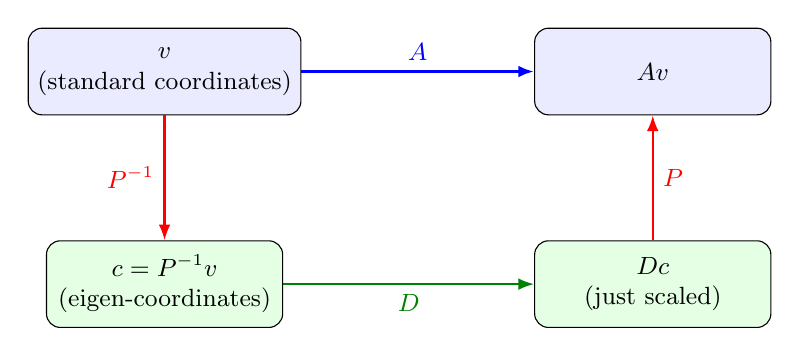
\begin{tikzpicture}[every node/.style={font=\small}, >={Latex[length=2mm]}]
	\node[draw, rounded corners=5pt, fill=blue!8, minimum width=3.0cm, minimum height=1.1cm, align=center] (v) at (0,2.7) {$v$\\ (standard coordinates)};
	\node[draw, rounded corners=5pt, fill=blue!8, minimum width=3.0cm, minimum height=1.1cm, align=center] (Av) at (6.2,2.7) {$Av$};
	\node[draw, rounded corners=5pt, fill=green!10, minimum width=3.0cm, minimum height=1.1cm, align=center] (c) at (0,0) {$c=P^{-1}v$\\ (eigen-coordinates)};
	\node[draw, rounded corners=5pt, fill=green!10, minimum width=3.0cm, minimum height=1.1cm, align=center] (Dc) at (6.2,0) {$Dc$\\ (just scaled)};
	\draw[->, very thick, blue] (v) -- (Av) node[midway, above] {$A$};
	\draw[->, thick, red] (v) -- (c) node[midway, left] {$P^{-1}$};
	\draw[->, thick, green!50!black] (c) -- (Dc) node[midway, below] {$D$};
	\draw[->, thick, red] (Dc) -- (Av) node[midway, right] {$P$};
\end{tikzpicture}
\end{document}
